\section{definition14-1(intergenerator diagram)}
\begin{definition}
\end{definition}

For every $n\in \mathbb{N}$, we define a local braid diagram inductively as follows:
We will call this braid diagram as inter-generator diagram on $n$ strands. It is a diagram that fits into the smaller disk in the figure below. It has $n$ red strands and $n$ blue strands where $n$ red strands start at $p_1 - p_n$ and end at $p'_1 - p'_n$, $n$ blue strands start at $q_1 - q_n$ and end at $q'_1 - q'_n$.

\begin{figure}[H] % Optional: [h] means here, [t] for top, [b] for bottom, [p] for page of floats
    \centering
    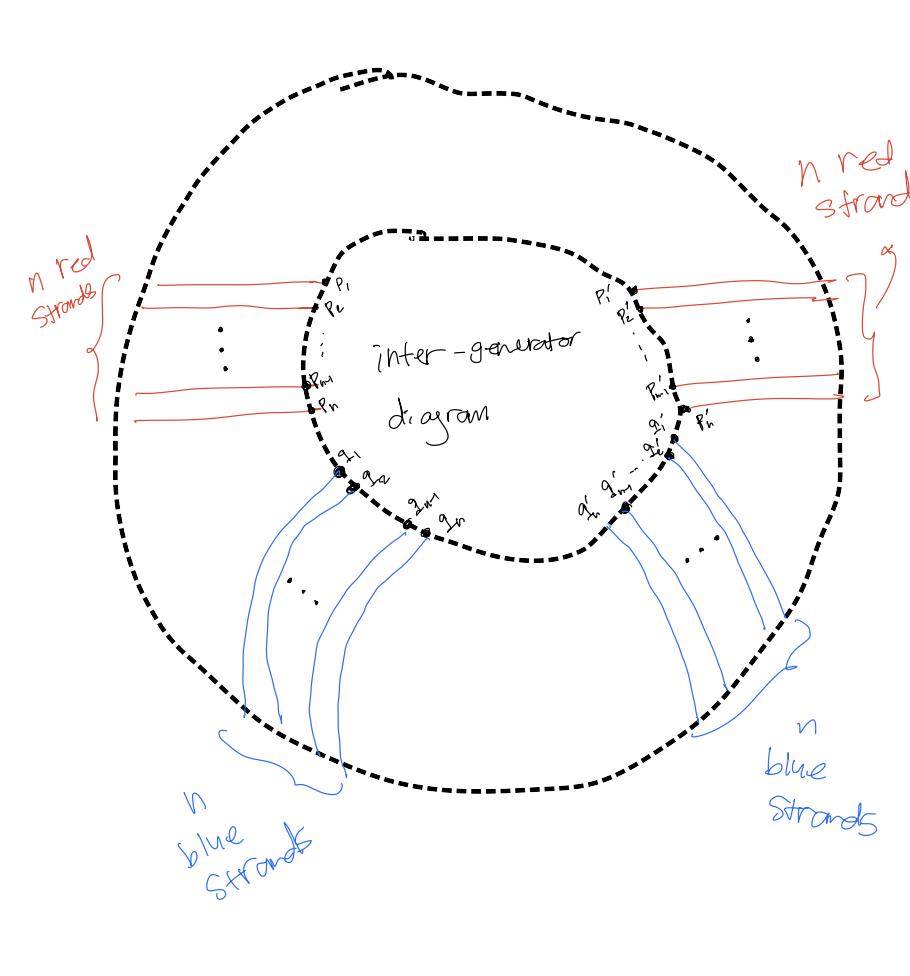
\includegraphics[width=\linewidth]{diagrams/definition14-1/1.png} % Adjust the width as needed
    \caption{Your caption here}
    \label{fig:your-label}
\end{figure}

If $n=1$, then the diagram is 

\begin{figure}[H] % Optional: [h] means here, [t] for top, [b] for bottom, [p] for page of floats
    \centering
    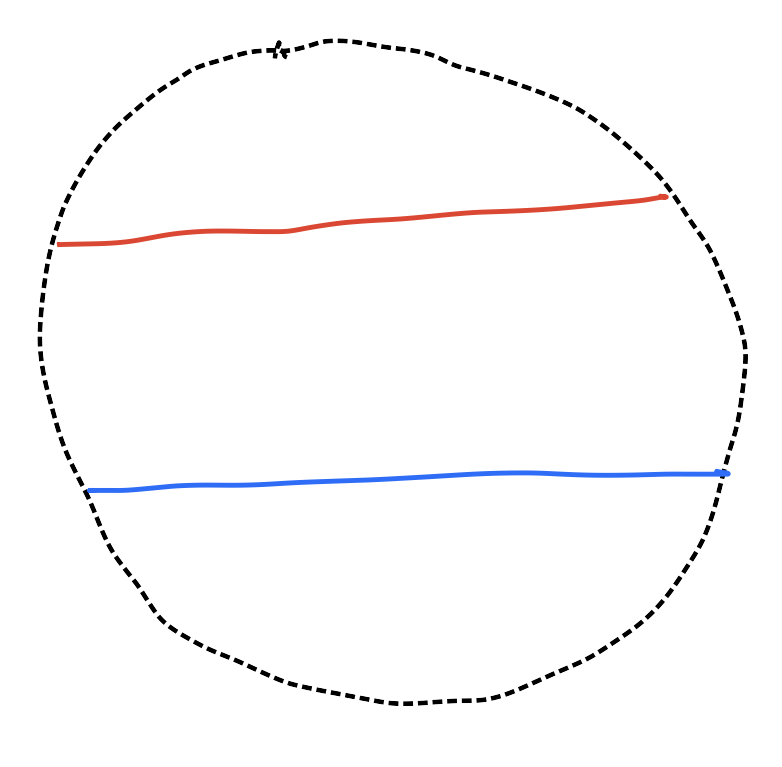
\includegraphics[width=\linewidth]{diagrams/definition14-1/2.png} % Adjust the width as needed
    \caption{Your caption here}
    \label{fig:your-label}
\end{figure}

Suppose we have defined inter-generator diagram up to $n-1$ strands. We define intergenerator diagram on $n$ strands as follows. To the following diagram :

\begin{figure}[H] % Optional: [h] means here, [t] for top, [b] for bottom, [p] for page of floats
    \centering
    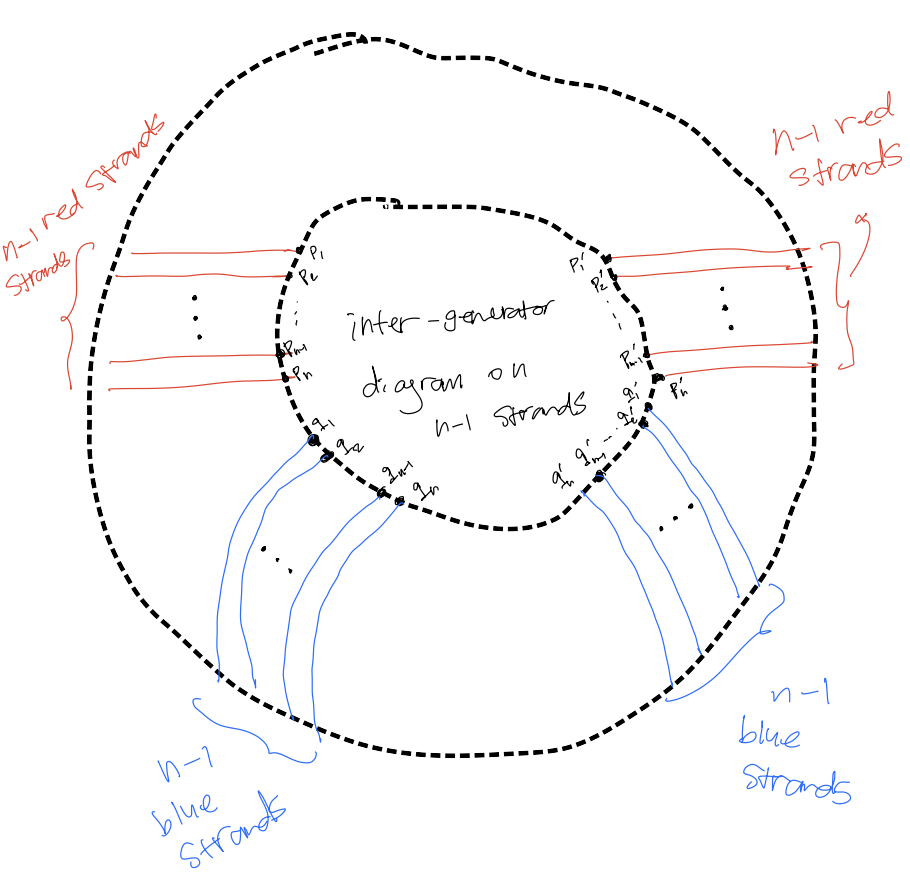
\includegraphics[width=\linewidth]{diagrams/definition14-1/3.png} % Adjust the width as needed
    \caption{Your caption here}
    \label{fig:your-label}
\end{figure}

we add a red strand and a blue strand as follows(drawn in thick lines)

\begin{figure}[H] % Optional: [h] means here, [t] for top, [b] for bottom, [p] for page of floats
    \centering
    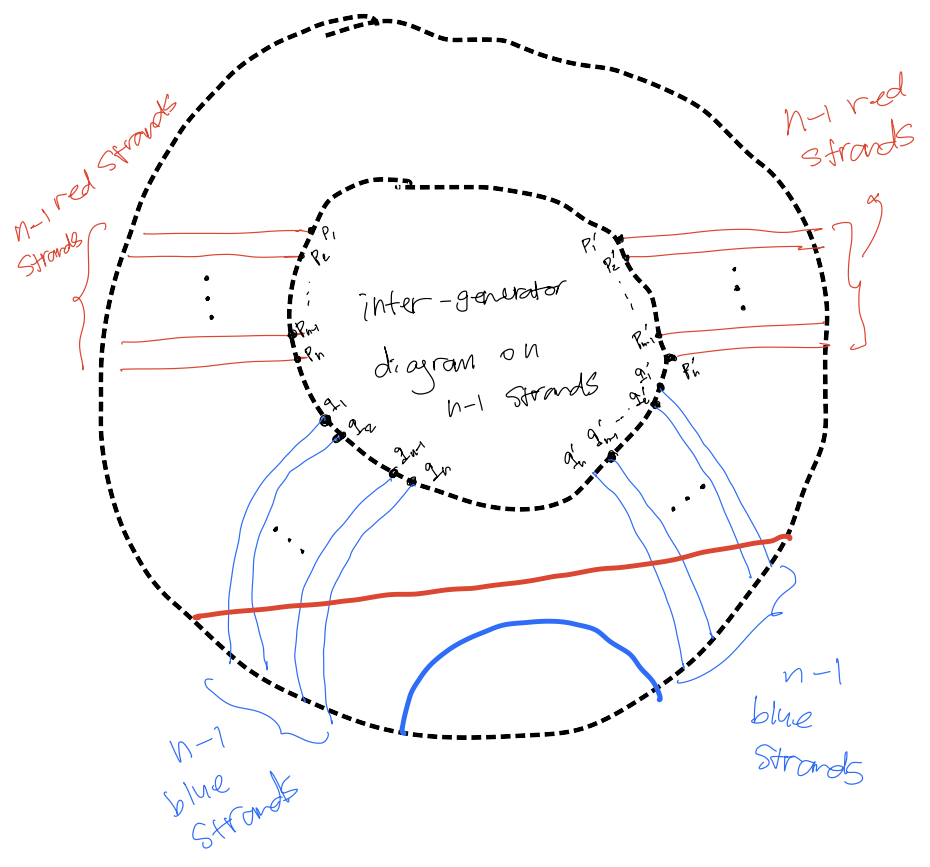
\includegraphics[width=\linewidth]{diagrams/definition14-1/4.png} % Adjust the width as needed
    \caption{Your caption here}
    \label{fig:your-label}
\end{figure}

NEw red strand is parallel to other red strands and crosses $n-1$ blue strand left and right. New blue strand does not cross any other lines.